% asparagines: 262 dash
% 332 dot
% 386 dash dot-dot
% 392 long-dash dot
% 448 solid
\begin{frame}[fragile]{OTFP Predicts DAVEI Activity Dependence on Linker Length}
\begin{tikzpicture}[scaleall=1.0]
\pcuad{\textwidth}{\textheight}
%\showcuad
\path(nw) ++(-0.75,0.15) node(text)[anchor=north west,text 
width=\textwidth]{{\tiny \textcolor{red!80!black}{S. Gossert and CFA, {\it Protein Science}, vol. 29, pp. 2304-2310, 2020. doi:10.1002/pro.3949}}};
\path(nw) ++(-0.75,-4) node(text2)[anchor=north west,text width=0.5\textwidth]{
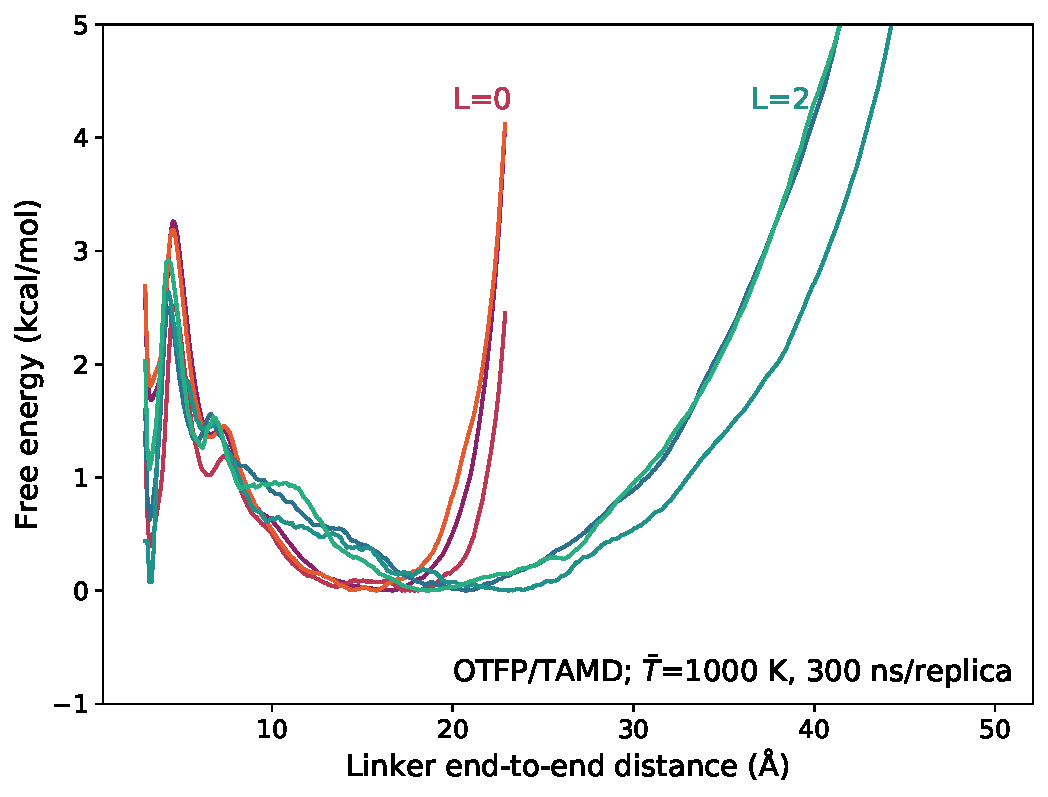
\includegraphics[width=\textwidth]{linker_pmf.pdf}};
\path(nw) ++(0.5,-0.15) node(text2)[anchor=north west,text width=0.4\textwidth]{
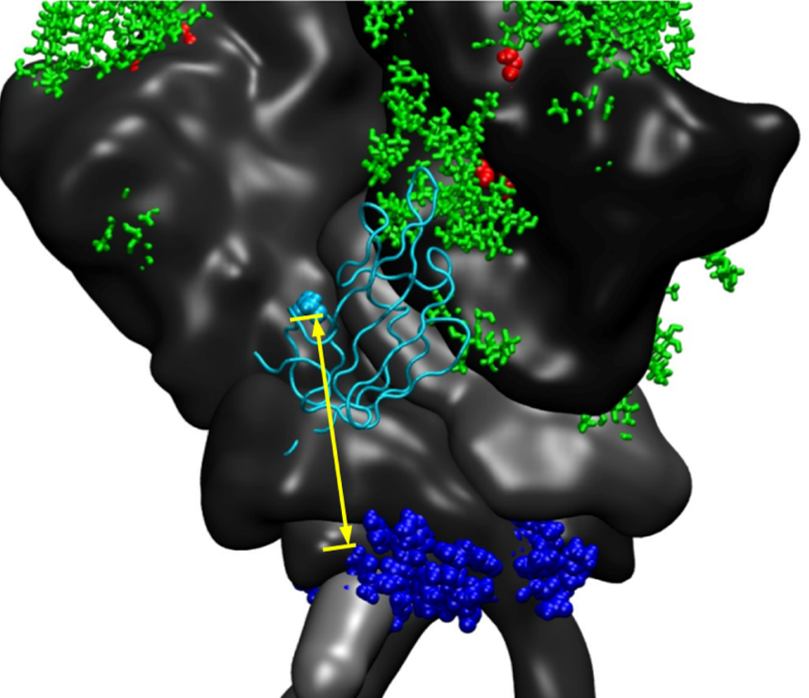
\includegraphics[width=\textwidth]{env+mvn_dist.png}};
\path(nw) ++(5,0) node(text2)[anchor=north west,text width=0.6\textwidth]{
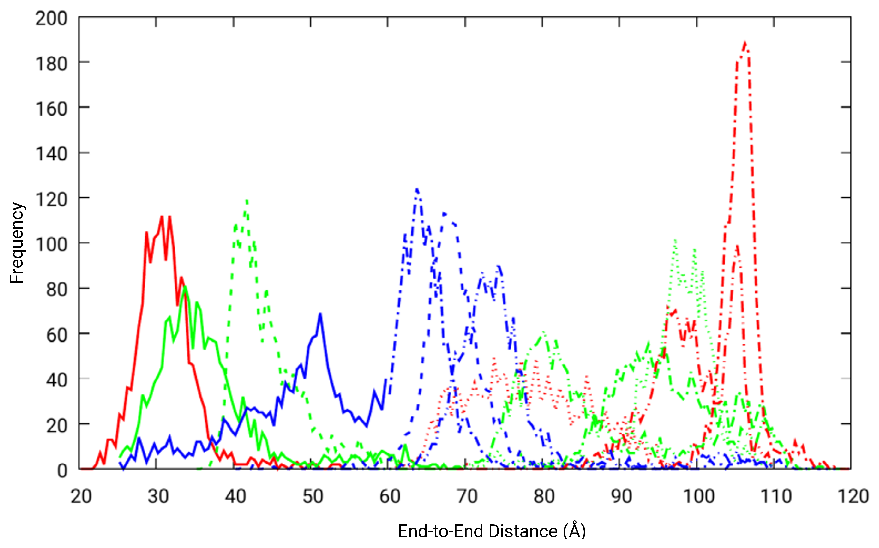
\includegraphics[width=\textwidth]{davei_env_mvn_dist_hist_1.png}};
\path(nw) ++(5.75,-0.25) node(text3)[anchor=north west,text width=0.5\textwidth]{\tiny MD, 40 ns};
\path(nw) ++(5.5,-4.25) node(text2)[anchor=north west,text width=0.45\textwidth]{
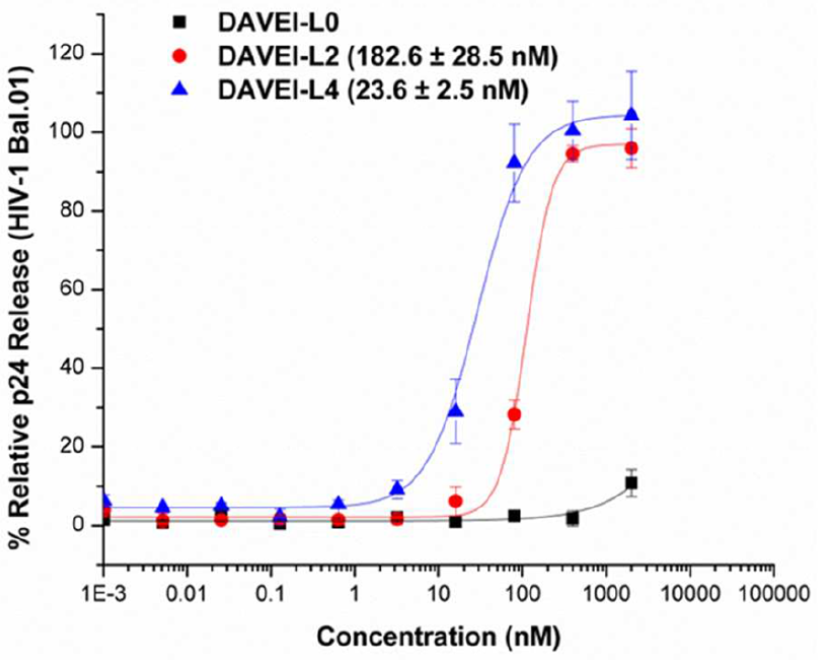
\includegraphics[width=\textwidth]{DAVEI-L02-experiment.png}};
\path(nw) ++(6.5,-0.5) node(text2)[anchor=north west,text width=0.1\textwidth]{
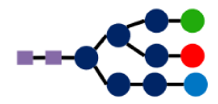
\includegraphics[width=\textwidth]{man9.png}};
\path(nw) ++(8.5,-0.4) node(text2)[anchor=north west,text width=0.08\textwidth]{

\includegraphics[width=\textwidth]{dashkey.png}};
\path(nw) ++(8.5,-0.25) node(text3)[anchor=north west,text width=0.5\textwidth]
{\tiny N-linked glycans};
\path(nw) ++(8.5,-0.4) node(text3)[anchor=north west,text width=0.5\textwidth]
{\tiny 262};
\path(nw) ++(8.5,-0.66) node(text3)[anchor=north west,text width=0.5\textwidth]
{\tiny 332};
\path(nw) ++(8.5,-0.92) node(text3)[anchor=north west,text width=0.5\textwidth]
{\tiny 386};
\path(nw) ++(8.5,-1.18) node(text3)[anchor=north west,text width=0.5\textwidth]
{\tiny 392};
\path(nw) ++(8.5,-1.48) node(text3)[anchor=north west,text width=0.5\textwidth]
{\tiny 448};
\path(nw) ++(-0.75,-1.5) node(label1)[anchor=north west,text width=0.4\textwidth]{MVN at\\N448 glycan};
\path(nw) ++(0.6,-2.4) node(label2)[anchor=north west,text width=0.2\textwidth]{40 \AA};
\path(nw) ++(-0.2,-3.2) node(label3)[anchor=north west,text width=0.4\textwidth]{Trp3 at MPER};
\end{tikzpicture}
\end{frame}

